
\section{Metodología}

    Crear una experiencia gamificada exitosa no solo consiste en aplicar mecánicas
    de juegos a una actividad específica, también requiere del seguimiento de un
    marco de instrucción apropiado \cite{GamInE-Learning}, razon por lo
    cual se decidió utilizan como principal referencia los marcos de trabajo
    {\it Octalysis} \cite{Octalysis} y {\it For The Win} \cite{ForTheWin}.\par
%
    \noindent 
    {\it Octalysis} define ocho principios de gamificación (diferenciación y
    pertenencia, desarrollo y recompensa, descubrimiento y retroalimentación,
    personalización, motivo e impulso social, codicia, impredecibilidad y curiosidad
    y miedo a la pérdida) los cuales representan distintas formas en las que se
    puede motivar a una persona a realizar una acción en específico, el marco de
    trabajo presenta cómo los principios trabajan en conjunto y proporciona técnicas
    específicas sobre cómo brindar soporte a cada uno de los principios.
%
    El segundo marco de trabajo utilizado es {\it For The Win}, el cual ofrece una
    guía pragmática que define una secuencia de pasos acerca de cómo implementar
    gamificación de forma correcta \cite{ForTheWin}. Además, describe el pensamiento
    de diseñador de juegos y establece una jerarquía entre los distintos elementos
    de juego (componentes, mecánicas y dinámicas) en la gamificación.\\
%
    El primer y segundo paso del marco {\it For The Win} consisten en definir
    los objetivos del sistema y delimitar las acciones de los usuarios, especificando
    el comportamiento que tendrán dentro del sistema \cite{ForTheWin}.
    Tomando en consideración ambos marcos de trabajo se detectaron 5 módulos
    principales a desarrollar sobre la plataforma de aprendizaje en linea de código
    abierto {\it Moodle}, el diagrama modular del sistema puede ser visto en la
    figura 1, a continuación se describen los módulos.\par
%
        \begin{center}
        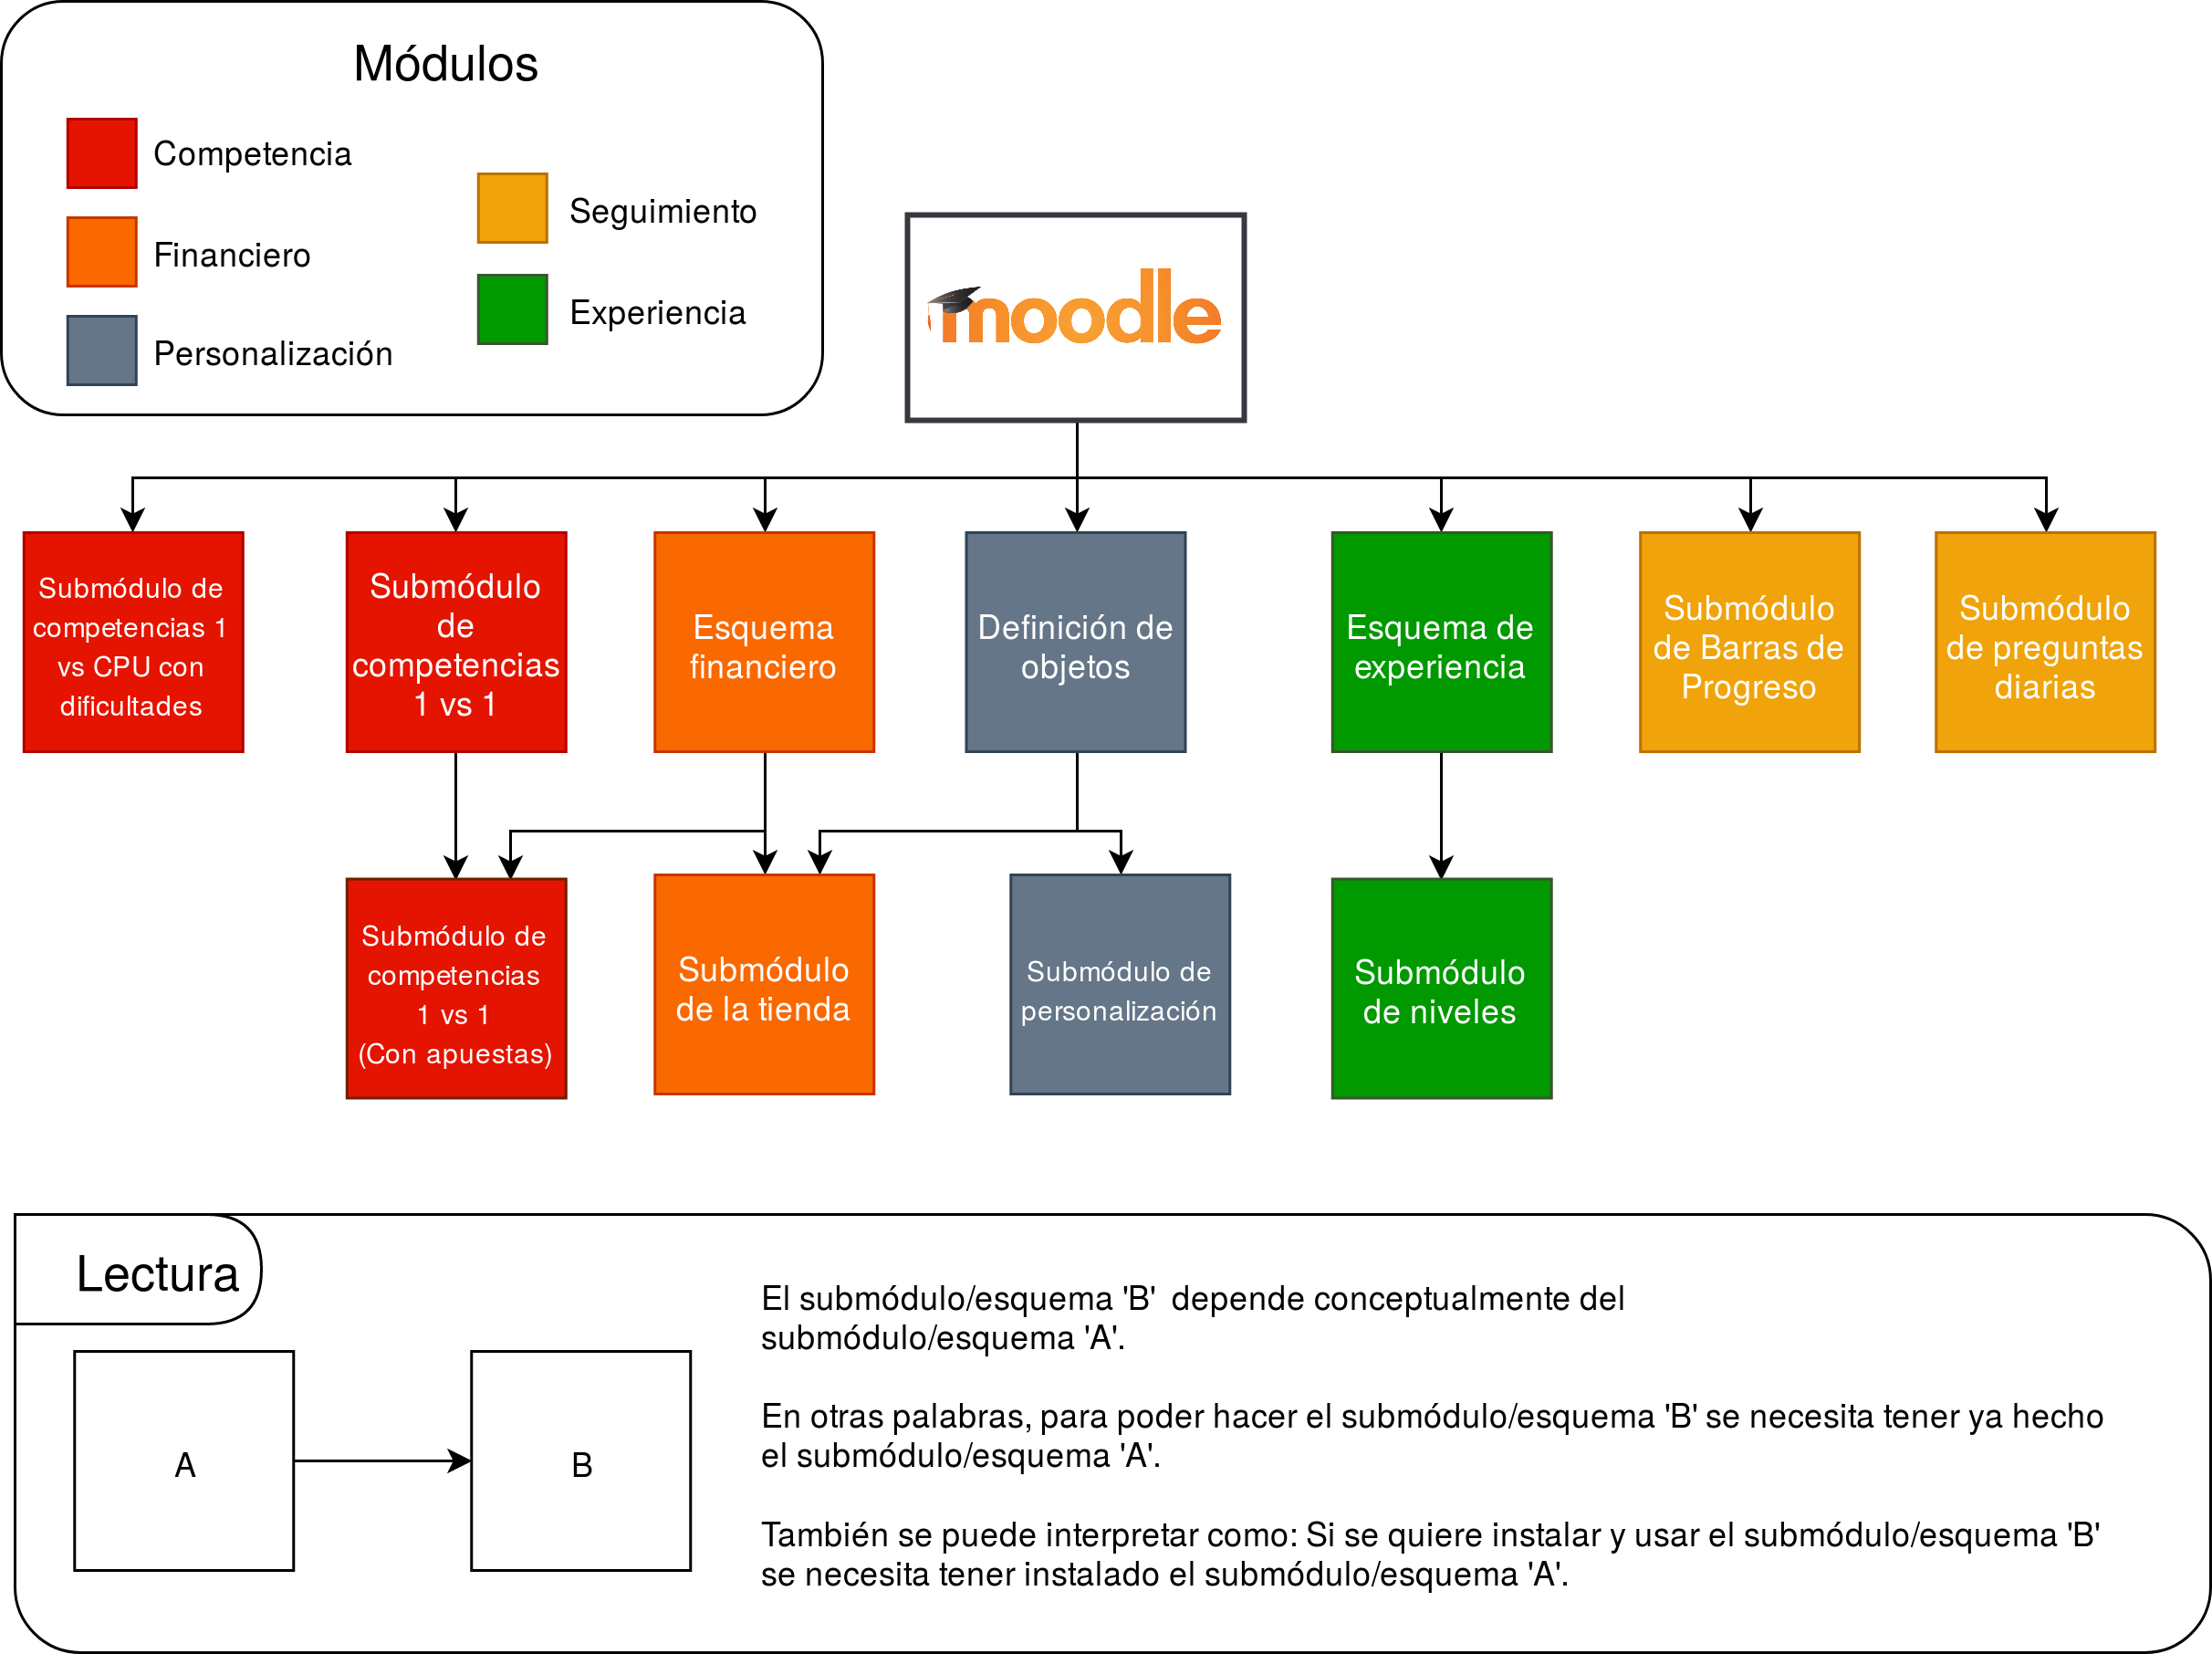
\includegraphics[width=1\linewidth]{images/modulos}
        \small Figura 1. Diseño modular del sistema.
        \end{center}
%
    {\it - Experiencia} brinda un mecanismo que permite a los usuarios medir su
    progreso como puntos de experiencia a nivel plataforma, además define la forma
    en que se obtienen los puntos de experiencia, la forma en que se visualiza la
    información, el número requerido para superar cada nivel y la barra de progreso
    del nivel actual.\\

    {\it - Competencia} brinda dos opciones para competir que otorgan al usuario
    la posibilidad de poner en práctica sus conocimientos del curso y a su vez
    interactuar con otros usuarios inscritos al curso.\\

    {\it - Personalización} pone a disposición de los usuarios una extensión a su
    perfil de moodle llamado ``perfil gamificado''. En el cual se puede seleccionar
    objetos para personalizar su perfil. Esta personalización es visible en los
    diferentes módulos de este proyecto que soporten esta función.\\

    {\it - Financiero} brinda un mecanismo que otorga la posibilidad a los usuarios
    de obtener monedas al realizar diferentes acciones en el sistema, con ellas puede
    adquirir los distintos elementos del módulo de personalización en el módulo
    de personalización.\\

    {\it - Seguimiento} permite a los usuarios tener un seguimiento de su progreso
    en el sistema. Lo cual otorga al usuario una manera de evaluar su rendimiento,
    mientras que le permite al profesor tener una actividad para que los alumnos
    contesten una pregunta de forma diaria.\\

% ==============================
    \noindent
    El siguiente paso o siguiente etapa consistió en definir los usuarios
    interactuarán con el sistema y construir las funcionalidades con base en los
    tipos de usuarios que lo usarán \cite{ForTheWin}. Los usuarios
    identificados son el {\it Administrador del sitio}, los {\it profesores} y
    {\it alumnos}. Con base a estos usuarios además de los requerimientos de cada se
    identificaron cuatro requerimientos generales los cuales son listados a
    continuación:\\

    {\it - Altamente configurale}
        Hace referencia a que se debe proporcionar al administrador, profesores
        y estudiantes la flexibilidad para que puedan configurar, habilitar o
        deshabilitar los distintos componentes que se desarrollarán dependiendo
        de las funcionalidades correspondientes a cada usuario.\\

    {\it - Instalación únicamente de elementos requeridos}
        Se debe brindar al administrador la opción de poder instalar únicamente
        los elementos que el requiera y de la misma forma, el profesor podrá escoger
        cuales desea incluir en sus cursos, finalmente el alumnos puede habilitar o
        deshabilitar los elementos visuales que no deseé ver.\\

    {\it - Bajo acoplamiento}
        El hecho de permitirle al administrador de la plataforma poder elegir los
        componentes que desea instalar, implica que los mismos deben estar
        diseñados para poder trabajar sin depender de las funciones de los demás
        componentes.\\

    {\it - Comunicación entre módulos}
        Hace referencia a que los eventos que ocurran en cada módulo puedan impulsar
        otros eventos o acciones en los demás módulos con la finalidad de que las
        distintas funcionalidades puedan trabajar en conjunto y se visualice como
        una única herramienta.\\

    \noindent
    El siguiente paso consiste en definir los ciclos de actividades o las etapas
    por las que pasa un usuario para avanzar en el sistema gamificado.
    \cite{ForTheWin}. Por lo que el administrador podrá instalar cualquiera
    de los módulos que deseé, en la siguiente etapa los profesores procederan a crear
    los cursos y con respecto a los cursos, diseñar y general el contenido incluyendo
    las funcionalidades específicas de gamificación que ellos requiran. Finalmente
    los alumons, dependiendo de las funcionalidades habilitadas por el administrador
    y por los profesores, realizará distintas actividades de forma repetitiva hasta
    alcanzar la meta, objetivo o completitud de las actividades de los cursos.\\

    \noindent
    El quinto consisten en diseñar el producto o sistema de forma apropiada para
    que este sea divertido, de acuerdo con {\it For The Win} para solventar este
    punto el diseño de los elementos de juego debe contemplar tanto elementos que
    apoyen a la motivación extrínseca cómo a la motivación intrínseca \cite%
    {ForTheWin}. Para llevar a cabo este punto se procedió vinculando los distintos
    módulos identificados con los principios de gamificación, estos módulos pueden
    ser vistos en la figura 2.

        \begin{center}
        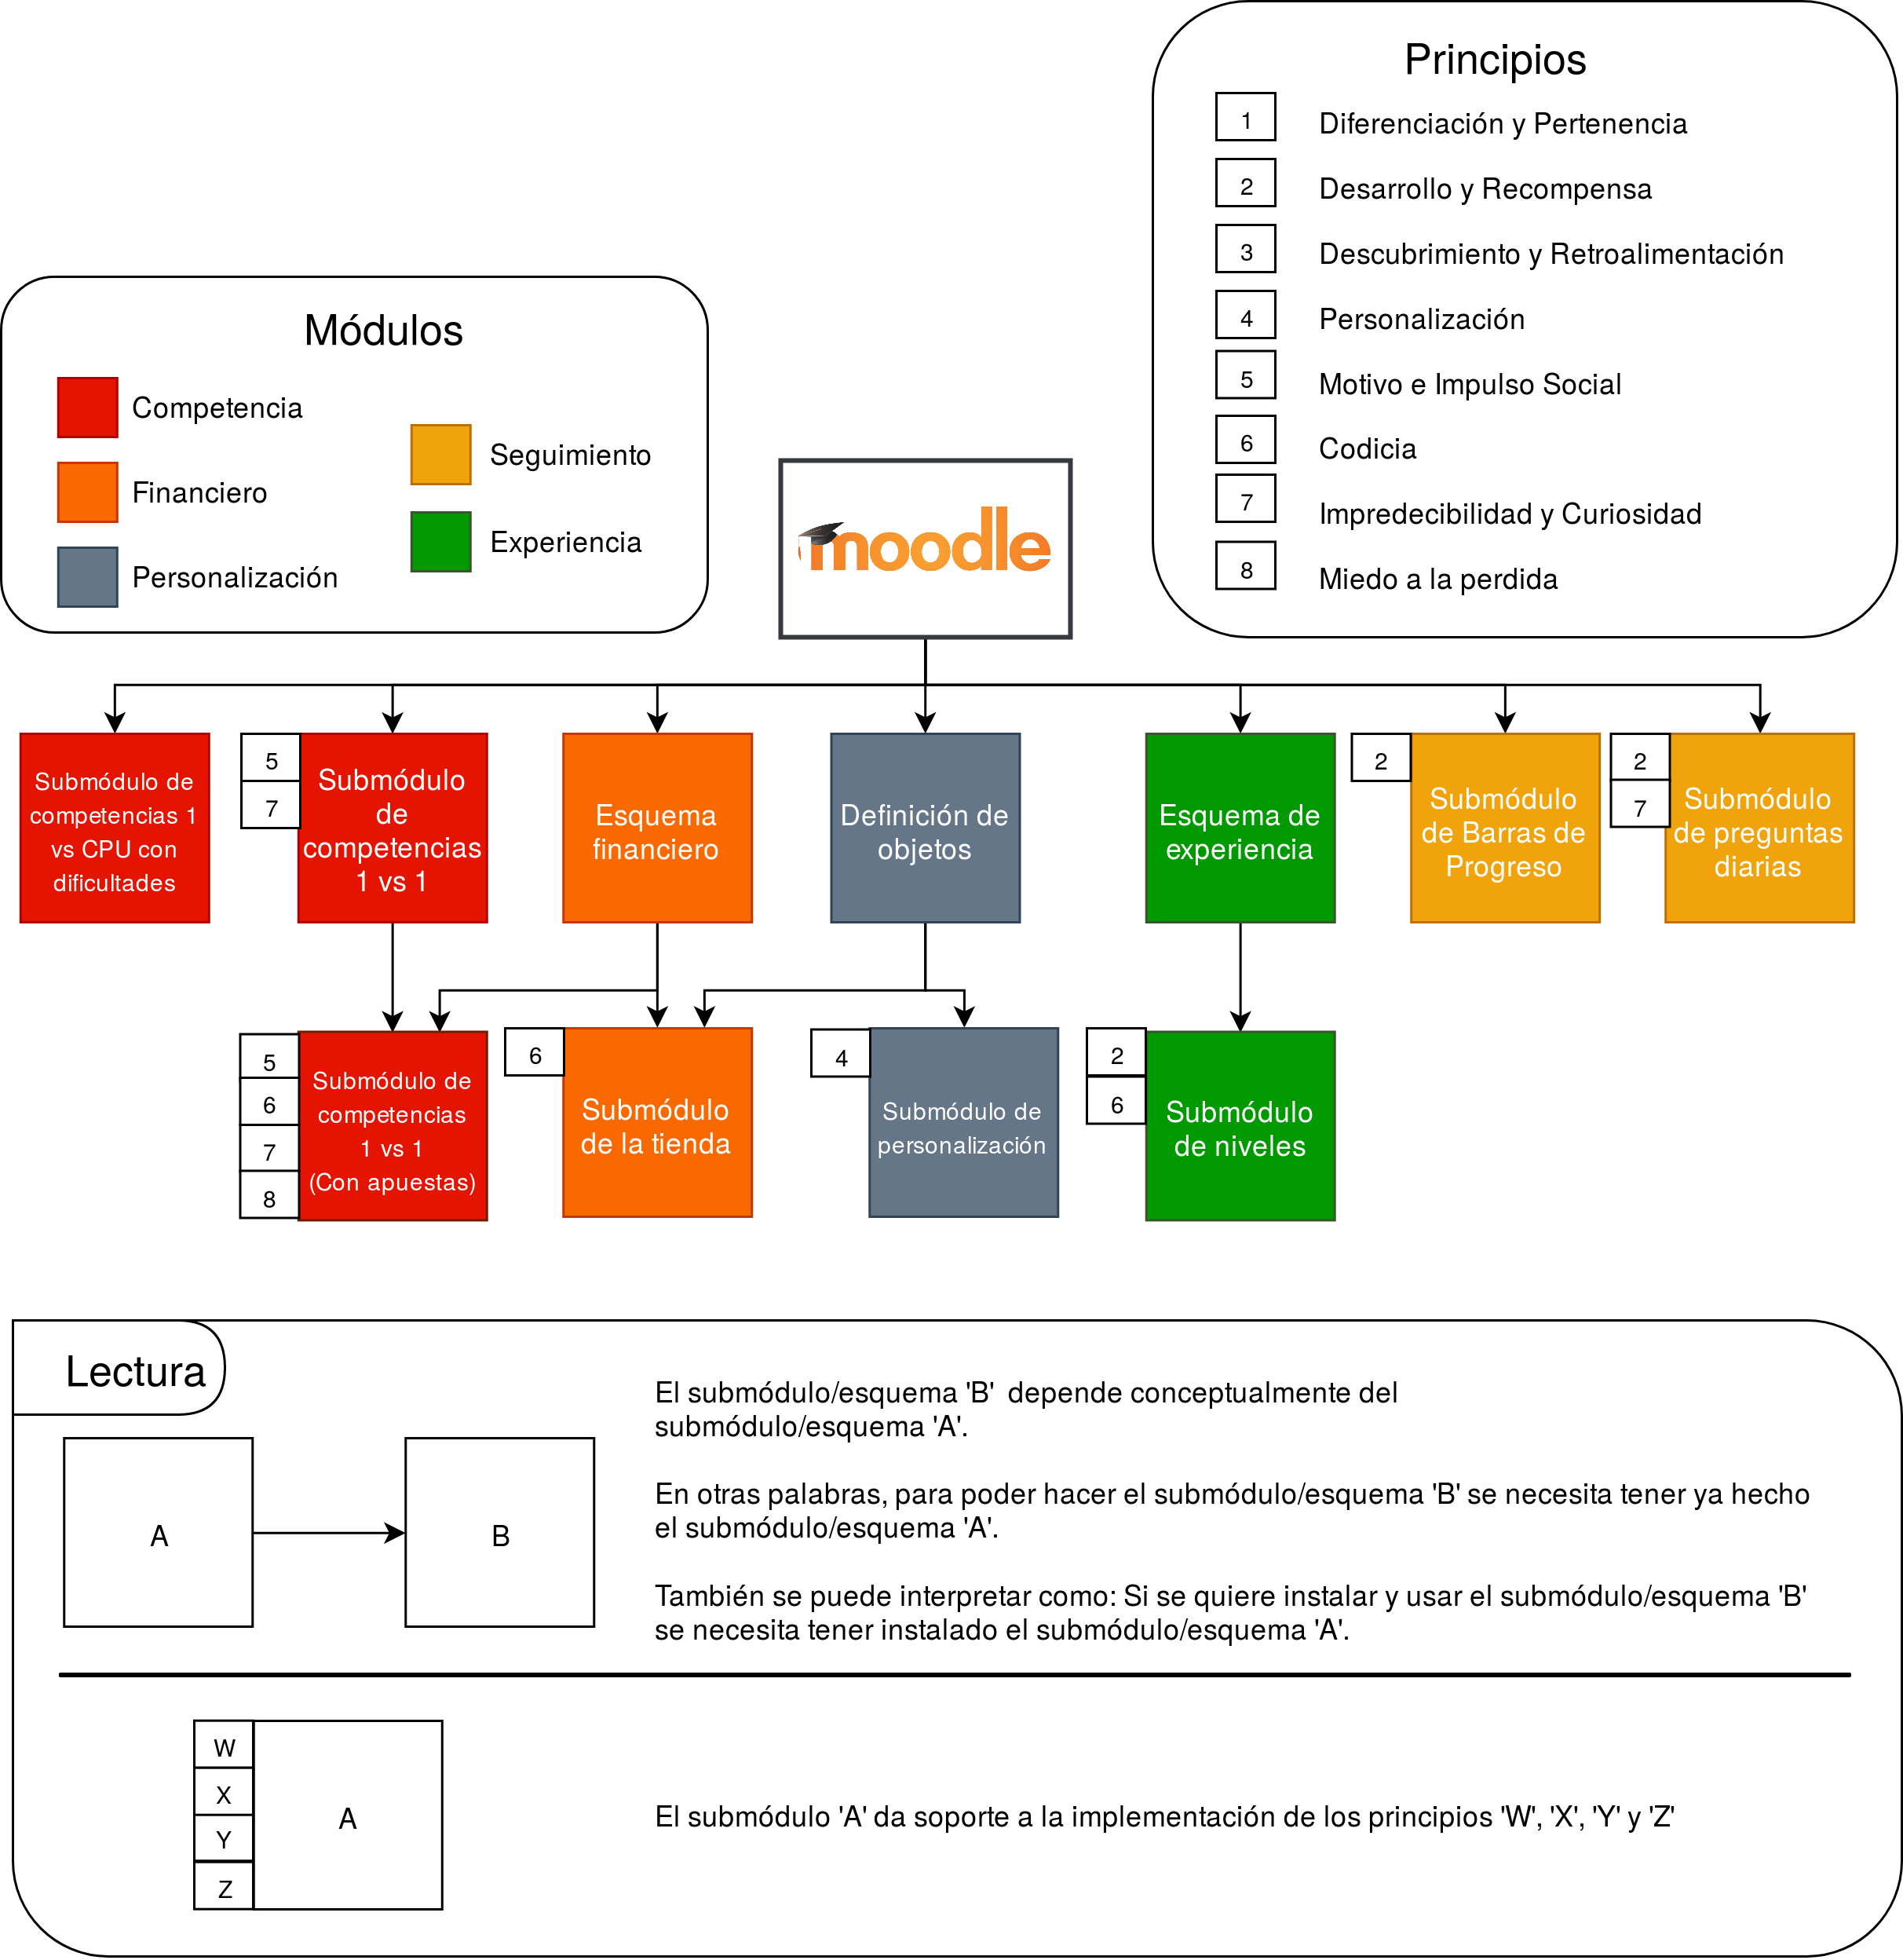
\includegraphics[width=1\linewidth]{images/modulosOctalysis}
        \small 2. Relación entre los módulos y los principios de gamificación.
        \end{center}

    En conjunto, los módulos identificados permiten brindar soporte a siete de los 
    ocho principios de gamificación (exceptuando el principio de descubrimiento y
    retroalimentación). De acuerdo con {\it Octalysis} \cite{Octalysis} los
    principios de gamificación estan relacionados con el tipo de motivación a la que
    brindan soporte, esta relación se muestra en la siguiente tabla. Con la relación
    entre los módulos identificados, los principios de {\it Octalysis} y tipos de
    motivación se brinda soporte a este punto. En la tabla mostrada a continuación
    los principios de gamificación se encuentran clasificados entre los que brindan
    soporte a la motivación intrínseca y extrínseca \cite{Octalysis}.\\

    \begin{center}
    \begin{tabular}{|p{0.4\linewidth}|p{0.4\linewidth}|} \hline
        {\bf Motivación intrínseca}  & {\bf Motivación Extrínseca} \\\hline
        Diferenciación y pertenencia & Diferenciación y pertenencia \\\hline
        Desarrollo y competencia     & Descubrimiento y retroalimentación \\\hline
        Personalización              & Motivo e Impulso social \\\hline
        Codicia                      & Impredecibilidad y curiosidad\\\hline
        Miedo a la pérdida           & Miedo a la pérdida\\\hline
    \end{tabular}\par\smallskip
    \small Tabla 1. Relación entre los tipos de motivación y los principios de
    Octalysis
    \end{center}

    \noindent
    Finalmente el último paso consiste en escoger específicamente que elementos
    de juego se deciden utilizar en el diseño del sistema, probarlos, ajustarlos y
    ejecutar los cambios requeridos para mejorar la implementación
    \cite{ForTheWin}. Este punto es tratado en parte del documento destinada
    al análisis, diseño y pruebas los módulos.\\

    {\it - Análisis}. El desarrollo del sistema se realizó de forma incrementan
    teniendo como iteración el desarrollo de cada módulo. El análisis de cada módulo
    consisten en identificar las funcionalidades específicas que este brindaría a cada
    uno de los usuarios, identificar las reglas de negocio y los casos de uso que
    describen las funcionalidades especificandolas como una transacción de valor
    entre el usuario y el sistema.\\

    {\it - Diseño}. Al igual que el análisis el diseño se realizó elaborando cuáles y
    cómo serían las interfaces de usuario nuevas, requeridas para el desarrollo de las
    nuevas funcionalidades. Además, respecto al diseño de la arquitectura se decidió
    que el desarrollo fuera mediante plugins debido a que brindan soporte a
    requerimientos generales descritos anteriormente. Los plugins diseñados se pueden
    encontrar en la figura 3.\par
%
    \noindent
    Se designó un plugin para ser el plugin central el cual tendría la única
    responsabilidad de especificar la forma en que se comunicarían los distintos
    plugins así como la responsabilidad de extender la esquema de base de datos de
    moodle con finalidad de establecer las relaciones del modelo de información usado
    en los distintos módulos.

        \begin{center}
        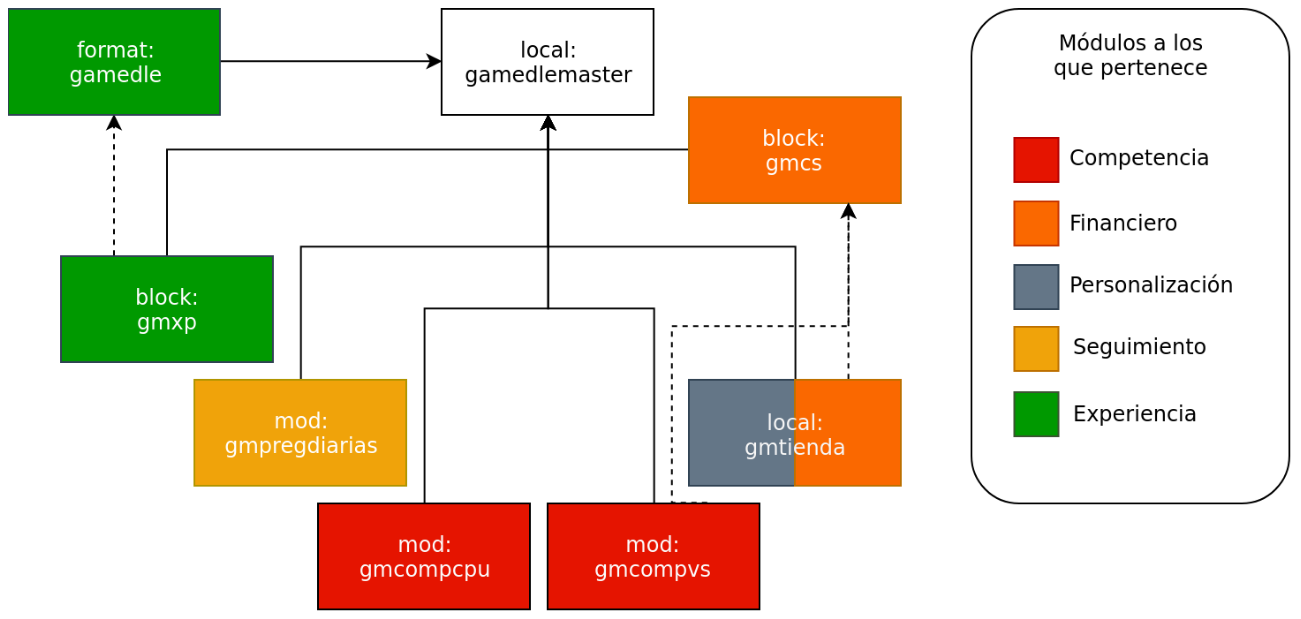
\includegraphics[width=1\linewidth]{images/plugins}
        \small Figura 3. Implementación de los módulos en plugins.
        \end{center}

    \noindent 
    Para el desarrollo de los demás plugins se buscó qué tipo de plugin sería el más
    adecuado para brindar la funcionalidad correspondiente al módulo, los tipos de
    plugins utilizados fuerón {\it bloques, plugin local, actividades y formato
    de curso}.\\

    {\it - Desarrollo} El desarrollo de cada uno de los plugins se llevo a cabo
    utilizando las distintas APIs que moodle brinda para el desarrollo de plugins, 
    cada una de estas API se centra en proveer una funcionalidad específica acerca
    de moodle, algunas de las APIs utilizadas fuerón: {\it DML (Data Management
    Language), DDL (Data Definition Language), Perfil de usuario, Configuraciones del
    administrador, Sistema de archivos, Fomularios, Navegación, API de páginas,
    módulos AMD (Asynchonous Module Definition), Completitud de cursos y actividades, 
    Eventos, entre otras}. El uso de cada una de estas APIs, requería adquirir el
    conocimeinto acerca de saber como utilizarla y en casos muy específicos saber como
    funcionaba internamente.\\

    {\it - Pruebas}
    La etapa de pruebas consistió en identificar los casos de prueba correspondientes
    a cada caso de uso elaborado, incluyendo casos de prueba correctos y casos de
    prueba incorrectos, dichos casos de prueba fueron probados conforme cada caso de 
    uso iba siendo desarrollado. En total se identificaron 77 casos de prueba para
    los cuales el desarrollo brinda soporte.\\

    Además de las pruebas de integración y funcionalidad se realizo una prueba de
    sistema donde alrededor de 15 estudiantes de la Escuela Superior de cómputo
    participaron resolviendo las actividades gamificadas que se encuentran dentro de
    un curso, especificamente el curso creado para la prueba contiene tres actividades
    principales del módulo de competencias.

